\section{Pulse Processing Electronics}
\subsection{General Concepts}
\begin{itemize}
    \item In the context of this course, signal amplification and shaping is done in analog then converted to digital  
    \item Signal processing and pulse-shape system\\
    See figure~\ref{fig:signal_processing}.
    \begin{figure}[ht]
        \centering
        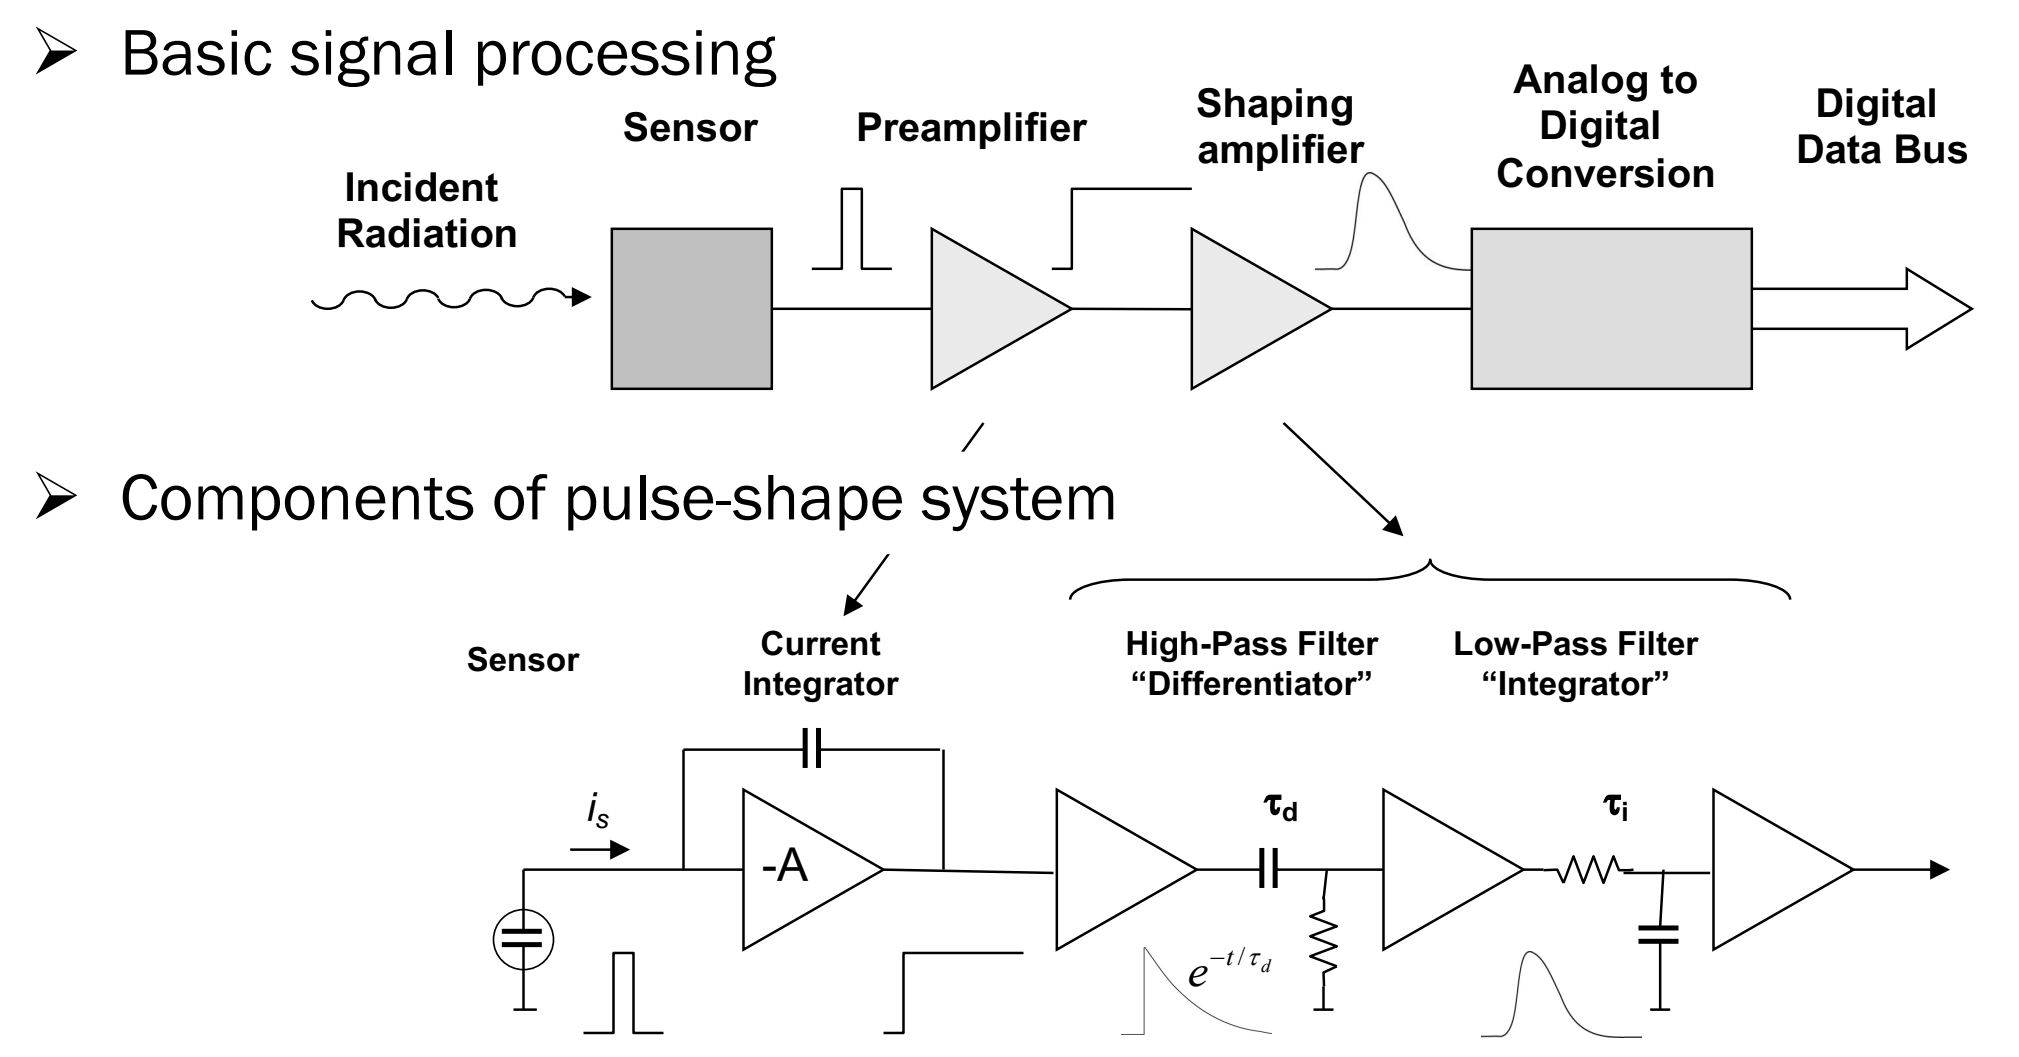
\includegraphics[width=0.8\textwidth]{images/signal_processing_diagram.png}
        \caption{Signal processing diagram.}
        \label{fig:signal_processing}
    \end{figure}
\end{itemize}
\subsection{Components}
\subsubsection{Preamplifier}

\subsubsection{Shaping ammplifier}
\subsubsection{Other components}
\subsection{Measurments of interest}
\subsubsection{Energy measurement}
\subsubsection{Time measurement}